\section{Parcours de graphes}

\frame{
    \frametitle{Ce qu'on veut faire}

    À partir d'un sommet $\sommet{}_0$ connu, déterminer les sommets d'un graphe $\graphe{}$ qui sont \enavant{atteignables} depuis $\sommet{}_0$, c'est-à-dire les sommets $\sommet{}$ tels qu'il existe un chemin de $\sommet{}_0$ à $\sommet{}$ dans $\graphe{}$. 
}

\subsection{Schéma générique}

\frame{
    \frametitle{Schéma générique d'exploration}

    \begin{columns}
        \begin{column}{5.5cm}
            \begin{description}
                \item[État initial~:] $\sommet{}_0$ est marqué\\ (c'est le seul)
                \item[Règle d'évolution~:] si $\sommet{}$ marqué et $\sommetb{}$ pas marqué et $(\sommet{}, \sommetb{})\in\arcs{}$, alors marquer $\sommetb{}$
                \item[État final~:]  plus aucune règle ne s'applique
            \end{description}
        \end{column}
        \begin{column}{5cm}
            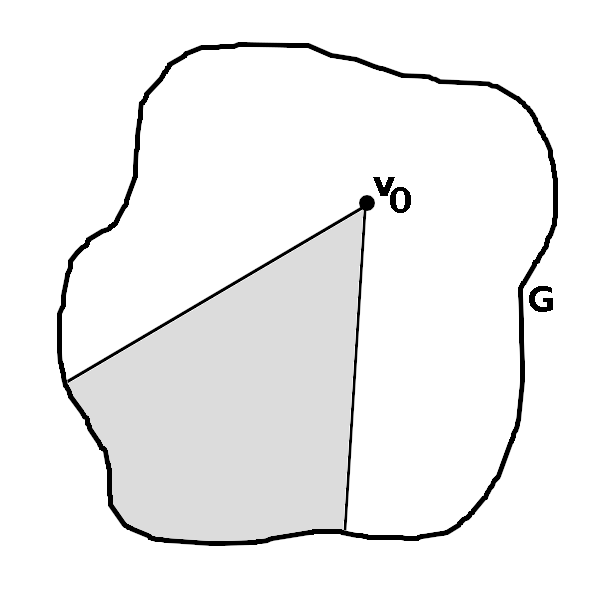
\includegraphics{schemagen.png}
        \end{column}
    \end{columns}
}

\frame{
    \frametitle{Propriétés}

    \proposition[sûreté]{%
        Si $\sommet{}$ est marqué alors il est atteignable depuis $\sommet{}_0$ (il existe un chemin de $\sommet{}_0$ à $\sommet{}$ dans $\graphe{}$)
    }

    \proposition[vivacité/terminaison]{%
        En appliquant la règle d'évolution en fini toujours par atteindre un état dans lequel il n'est plus possible de l'appliquer.
    }

    \proposition[complétude]{%
        Dans un état final, tout sommet atteignable depuis $\sommet{}_0$ est marqué.
    }

    \pause

    \exercice{%
        Prouver ces trois propositions.
    }
}

\subsection{Algorithme de parcours}

\frame{
    \frametitle{Le tas, une structure de données générique}

    \begin{block}{Interface}
        \begin{description}
            \item[init] créer un tas vide
            \item[ajouter] ajouter un élément dans le tas
            \item[observer] obtenir un élément du tas 
            \item[extraire] enlever un élément du tas
            \item[estVide] vérifier s'il reste des éléments dans le tas 
        \end{description}
    \end{block}

    Si le tas n'a pas changé entre observer et extraire, \enavant{l'élément qui est enlevé du tas doit être celui qui avait été obtenu}.

    \begin{exampleblock}{Exemple}
        \begin{center}
            \begin{minipage}{5cm}
                \begin{algorithmic}
                    \State $t = init()$
                    \State $t.ajouter(5)$
                    \If{$!t.estVide()$}
                        \State $v = t.observer()$
                        \State $t.extraire()$
                    \EndIf
                \end{algorithmic}
            \end{minipage}
        \end{center}
    \end{exampleblock}
}

\frame{
    \frametitle{Algorithme de parcours générique}

    \begin{columns}
        \begin{column}{7cm}
            \begin{center}
                \begin{minipage}{7cm}
                    \begin{algorithmic}
                        \In{$\graphedef{}$, $\sommet{}_0\in\sommets{}$}
                        \Out{???}
                        \State $t = init()$
                        \State $t.ajouter(\sommet{}_0)$
                        \State marquer $\sommet{}_0$
                        \While{$!t.estVide()$}
                            \State $v = t.observer()$
                            \If{$\exists (\sommet{}, \sommetb{})\in \arcs{}$, $\sommetb{}$ non marqué}
                                \State $t.ajouter(\sommetb{})$
                                \State marquer $\sommetb{}$
                            \Else
                                \State $t.extraire()$
                            \EndIf
                        \EndWhile
                    \end{algorithmic}
                \end{minipage}
            \end{center}
        \end{column}
        \begin{column}{4cm}
            \pause

            \exercice{%
                Effectuer un parcours du graphe suivant à partir de $v_0 = v_1$
                \begin{center}
                    \scalebox{0.8}{
                        \begin{tikzpicture}
                            \node (a) at (0,0) {$\sommet{}_3$};
                            \node (b) at (3,0) {$\sommet{}_4$};
                            \node (c) at (0,3) {$\sommet{}_1$};
                            \node (d) at (3,3) {$\sommet{}_2$};

                            \shiftdraw{d}{a}{-1pt}{1pt};
                            \draw[-latex] (a) to[in=270, out=180, looseness=5] (a);

                            \shiftdraw{c}{d}{0}{1.5pt};

                            \shiftdraw{d}{b}{-1.5pt}{0};
                        \end{tikzpicture}
                    }
                \end{center}
            }
        \end{column}
    \end{columns}
}

\frame{
    \frametitle{Propriétés de l'algorithme de parcours générique}

    \proposition{%
        Tout sommet dans le tas est marqué.
    }

    \proposition[sûreté]{%
        Si $\sommet{}$ est marqué alors $\sommet{}$ est atteignable depuis $\sommet{}_0$.
    }

    \proposition[vivacité/terminaison]{%
        À un moment, le tas est vide.
    }

    \proposition[complétude]{%
        Quand le tas est vide tous les sommets atteignables sont marqués.
    }

    \pause

    \exercice{%
        Prouver ces quatre propositions.
    }
}

\subsection{Parcours en largeur}

\frame{
    \frametitle{Un tas particulier : la file}

    Structure \enavant{FIFO} (First In, First Out)

    \begin{center}
        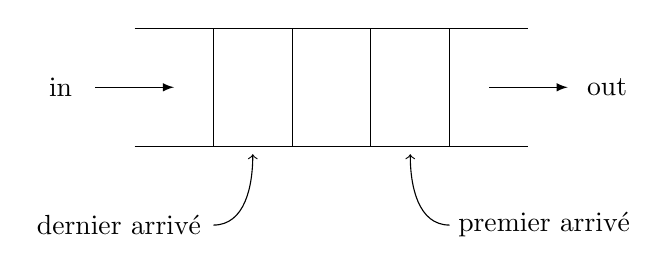
\begin{tikzpicture}
            \draw (0,0) -- (5,0);
            \draw (0,1.5) -- (5,1.5);
            \draw (1,0) -- (1,1.5);
            \draw (2,0) -- (2,1.5);
            \draw (3,0) -- (3,1.5);
            \draw (4,0) -- (4,1.5);
            \draw[-latex] (-0.5,0.75) -- (0.5,0.75);
            \draw[-latex] (4.5,0.75) -- (5.5,0.75);
            \node (tmp) at (-1, 0.75) {~in};
            \node (tmp) at (6, 0.75) {out};
            \draw[->] (1,-1) to[out=0, in=270] (1.5, -0.1);
            \draw[->] (4,-1) to[out=180, in=270] (3.5, -0.1);
            \node (tmp) at (-0.2, -1) {dernier arrivé};
            \node (tmp) at (5.2, -1) {premier arrivé};
        \end{tikzpicture}
    \end{center}

    \begin{block}{Interface}
        \begin{description}
            \item[ajouter] mettre un élément à la fin de la file
            \item[observer] obtenir le premier élément dans la file
            \item[extraire] retirer le premier élément de la file 
        \end{description}
    \end{block}
}

\frame{
    \frametitle{Parcours en largeur (Breadth-First Search)}

    Si on utilise une \enavant{file} pour implanter l'algorithme de parcours générique précédent on obtient un parcours particulier appelé \enavant{parcours en largeur} (aussi appelé en largeur d'abord).

    \exercice{%
        Effectuer un parcours en largeur du graphe suivant à partir de $v_0 = v_1$
        \begin{center}
            \begin{tikzpicture}
                \node (a) at (0,0) {$\sommet{}_3$};
                \node (b) at (3,0) {$\sommet{}_4$};
                \node (c) at (0,3) {$\sommet{}_1$};
                \node (d) at (3,3) {$\sommet{}_2$};

                \shiftdraw{d}{a}{-1pt}{1pt};
                \draw[-latex] (a) to[in=270, out=180, looseness=5] (a);

                \shiftdraw{c}{d}{0}{1.5pt};

                \shiftdraw{d}{b}{-1.5pt}{0};
            \end{tikzpicture}
        \end{center}
    }
}

\frame{
    \frametitle{Propriété fondamentale du parcours en largeur}

    \definition[plus court chemin]{%
        Soit $\graphedef{}$ un graphe, soient $\sommet{}$ et $\sommetb{}$ deux sommets de $\graphe{}$.
        Un chemin $\chemin{}$ de $\sommet{}$ à $\sommetb{}$ est un plus court chemin de $\sommet{}$ à $\sommetb{}$ si tout autre chemin $\chemin{}'$ de $\sommet{}$ à $\sommetb{}$ est tel que $\taille{\chemin{}'} \geq \taille{\chemin{}}$.
    }

    \definition[distance]{%
        On appelle distance de $\sommet{}$ à $\sommetb{}$ la longueur d'un plus court chemin de $\sommet{}$ à $\sommetb{}$.
        On la note $\distance{\sommet{}}{\sommetb{}}$.
    }

    \pause

    \proposition{%
        Durant un parcours en largeur, à tout instant, si $\sommet{}$ est marqué alors tous les sommets $\sommetb{}$ tels que $\distance{\sommet{}_0}{\sommetb{}} < \distance{\sommet{}_0}{\sommet{}}$ le sont déjà.
    }
}

\frame{
    \frametitle{Propriété fondamentale du parcours en largeur, suite}

    Conséquence de la proposition~: on découvre les sommets (on les marque) dans l'ordre de leur distance à $\sommet{}_0$.

    \begin{center}
        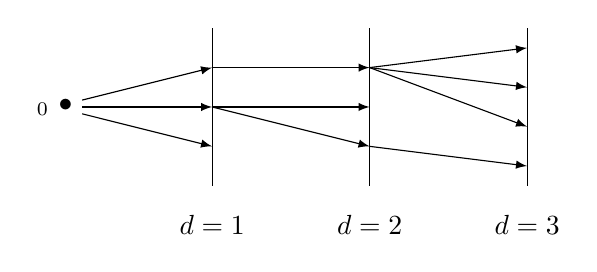
\begin{tikzpicture}
            \node (v0) at (-1,0) {$\sommet{}_0 ~\bullet$};
            \draw (1,1) -- (1,-1);
            \draw (3,1) -- (3,-1);
            \draw (5,1) -- (5,-1);
            \node (tmp) at (1,-1.5) {$d=1$};
            \node (tmp) at (3,-1.5) {$d=2$};
            \node (tmp) at (5,-1.5) {$d=3$};
            \draw[-latex] (v0) -- (1,0.5);
            \draw[-latex] (v0) -- (1,0);
            \draw[-latex] (v0) -- (1,-0.5);
            \draw[-latex] (1,0.5) -- (3,0.5);
            \draw[-latex] (1,0) -- (3,0);
            \draw[-latex] (1,0) -- (3,-0.5);
            \draw[-latex] (3,0.5) -- (5,0.75);
            \draw[-latex] (3,0.5) -- (5,0.25);
            \draw[-latex] (3,0.5) -- (5,-0.25);
            \draw[-latex] (3,-0.5) -- (5,-0.75);
        \end{tikzpicture}
    \end{center}

    \pause

    \exercice{%
        Prouver la proposition (on peut le faire par l'absurde).
    }
}

\frame{
    \frametitle{Parcours en largeur, autre version}

    \begin{center}
        \begin{minipage}{8.5cm}
            \begin{algorithmic}
                \In{$\graphedef{}$, $\sommet{}_0\in\sommets{}$}
                \only<2->{\Out{\enavant{pred}}}
                \State $t = init()$
                \State $t.ajouter(\sommet{}_0)$
                \State marquer $\sommet{}_0$
                \While{$!t.estVide()$}
                    \State $v = t.observer()$
                    \State $t.extraire()$
                    \ForAll{$\sommetb{}$ t.q $\exists (\sommet{}, \sommetb{})\in \arcs{}$, $\sommetb{}$ non marqué}
                        \State $t.ajouter(\sommetb{})$
                        \State marquer $\sommetb{}$
                        \only<2->{\State \enavant{$pred(\sommetb{}) = \sommet{}$}}
                    \EndFor
                \EndWhile
            \end{algorithmic}
        \end{minipage}
    \end{center}

    \only<2->{
        \proposition{%
            pred définit un routage par des plus courts chemins depuis $\sommet{}_0$ vers les sommets marqués.
        }
    }
}

\frame{
    \frametitle{Parcours en largeur, exercice et preuve}

    \exercice{%
        \begin{columns}
            \begin{column}{7cm}
                Soit le graphe suivant~:
                \begin{tikzpicture}
                    \node (v4) at (0,0) {$\sommet{}_4$};
                    \node (v5) at (3,0) {$\sommet{}_5$};
                    \node (v1) at (0,3) {$\sommet{}_1$};
                    \node (v2) at (3,3) {$\sommet{}_2$};
                    \node (v3) at (6,1.5) {$\sommet{}_3$};

                    \shiftdraw{v1}{v2}{0}{0};
                    \shiftdraw{v2}{v3}{0}{0};
                    \shiftdraw{v4}{v1}{0}{0};
                    \shiftdraw{v5}{v4}{0}{0};
                    \shiftdraw{v5}{v3}{0}{0};

                    \draw[-latex] (v2) to[in=45, out=135, looseness=5] (v2);
                \end{tikzpicture}
            \end{column}
            \begin{column}{4cm}
                \begin{itemize}
                    \item Faire pas à pas le parcours en largeur de ce graphe à partir de $\sommet{}_0 = \sommet{}_1$ et en calculant pred.
                    \item En déduire le plus court chemin de $\sommet{}_1$ à $\sommet{}_3$.
                \end{itemize}
            \end{column}
        \end{columns}
    }

    \pause

    \exercice{%
        Faire la preuve de la proposition précédente.
        On peut commencer par montrer que pred définit un routage et montrer ensuite que ce routage est par des plus courts chemins.
    }
}

\subsection{Parcours en profondeur}

\frame{
    \frametitle{Un tas particulier : la pile}

    Structure \enavant{LIFO} (Last In, First Out)

    \begin{columns}
        \begin{column}{5cm}
            \begin{center}
                \begin{tikzpicture}
                    \draw (0,0) -- (0,4.5);
                    \draw (2,0) -- (2,4.5);
                    \draw (0,0) -- (2,0);
                    \draw (0,1) -- (2,1);
                    \draw (0,2) -- (2,2);
                    \draw (0,3) -- (2,3);
                    \draw[-latex] (0.6,5) -- (0.6,4);
                    \draw[-latex] (1.4,4) -- (1.4,5);
                    \node (tmp) at (0.6, 5.25) {in};
                    \node (tmp) at (1.4, 5.25) {out};
                    \draw[->] (3,3.5) to[out=270, in=0] (2.1, 2.5);
                    \draw[->] (3,-0.5) to[out=90, in=0] (2.1, 0.5);
                    \node (tmp) at (3.5, 3.8) {dernier arrivé};
                    \node (tmp) at (3.5, -0.8) {premier arrivé};
                \end{tikzpicture}
            \end{center}
        \end{column}
        \begin{column}{6cm}
            \begin{block}{Interface}
                \begin{description}
                    \item[ajouter] mettre un élément au sommet de la pile
                    \item[observer] obtenir l'élément au sommet de la pile
                    \item[extraire] retirer l'élément au sommet de la pile
                \end{description}
            \end{block}
        \end{column}
    \end{columns}
}

\frame{
    \frametitle{Parcours en profondeur (Depth-First Search)}

    Si on utilise une \enavant{pile} pour implanter l'algorithme de parcours générique précédent on obtient un parcours particulier appelé \enavant{parcours en profondeur} (aussi appelé en profondeur d'abord).

    \exercice{%
        Effectuer un parcours en profondeur du graphe suivant à partir de $v_0 = v_1$
        \begin{center}
            \begin{tikzpicture}
                \node (a) at (0,0) {$\sommet{}_3$};
                \node (b) at (3,0) {$\sommet{}_4$};
                \node (c) at (0,3) {$\sommet{}_1$};
                \node (d) at (3,3) {$\sommet{}_2$};

                \shiftdraw{d}{a}{-1pt}{1pt};
                \draw[-latex] (a) to[in=270, out=180, looseness=5] (a);

                \shiftdraw{c}{d}{0}{1.5pt};

                \shiftdraw{d}{b}{-1.5pt}{0};
            \end{tikzpicture}
        \end{center}
    }
}

\frame{
    \frametitle{Propriétés du parcours en profondeur}

    \proposition{%
        À tout instant la pile (si elle n'est pas vide) définit un chemin de $\sommet{}_0$ au sommet $\sommet{}$ situé à son sommet.
    }

    \exercice{%
        Le prouver.
    }

    \pause

    \proposition{%
        Si $\sommet{}$ est dépilé, alors tous les sommets $\sommetb{}$ atteignables depuis $\sommet{}$ par un chemin $\sommet{}\cheminvers{}\sommetb{}$ ne passant par aucun sommet encore dans la pile sont marqués.
    }

    \exercice{%
        Le prouver.
    }
}